\documentclass{standalone}
\usepackage{tikz}
\usetikzlibrary{patterns, positioning}
\usepackage[sfdefault]{ClearSans} %% option 'sfdefault' activates Clear Sans as the default text font
\usepackage[T1]{fontenc}

\begin{document}
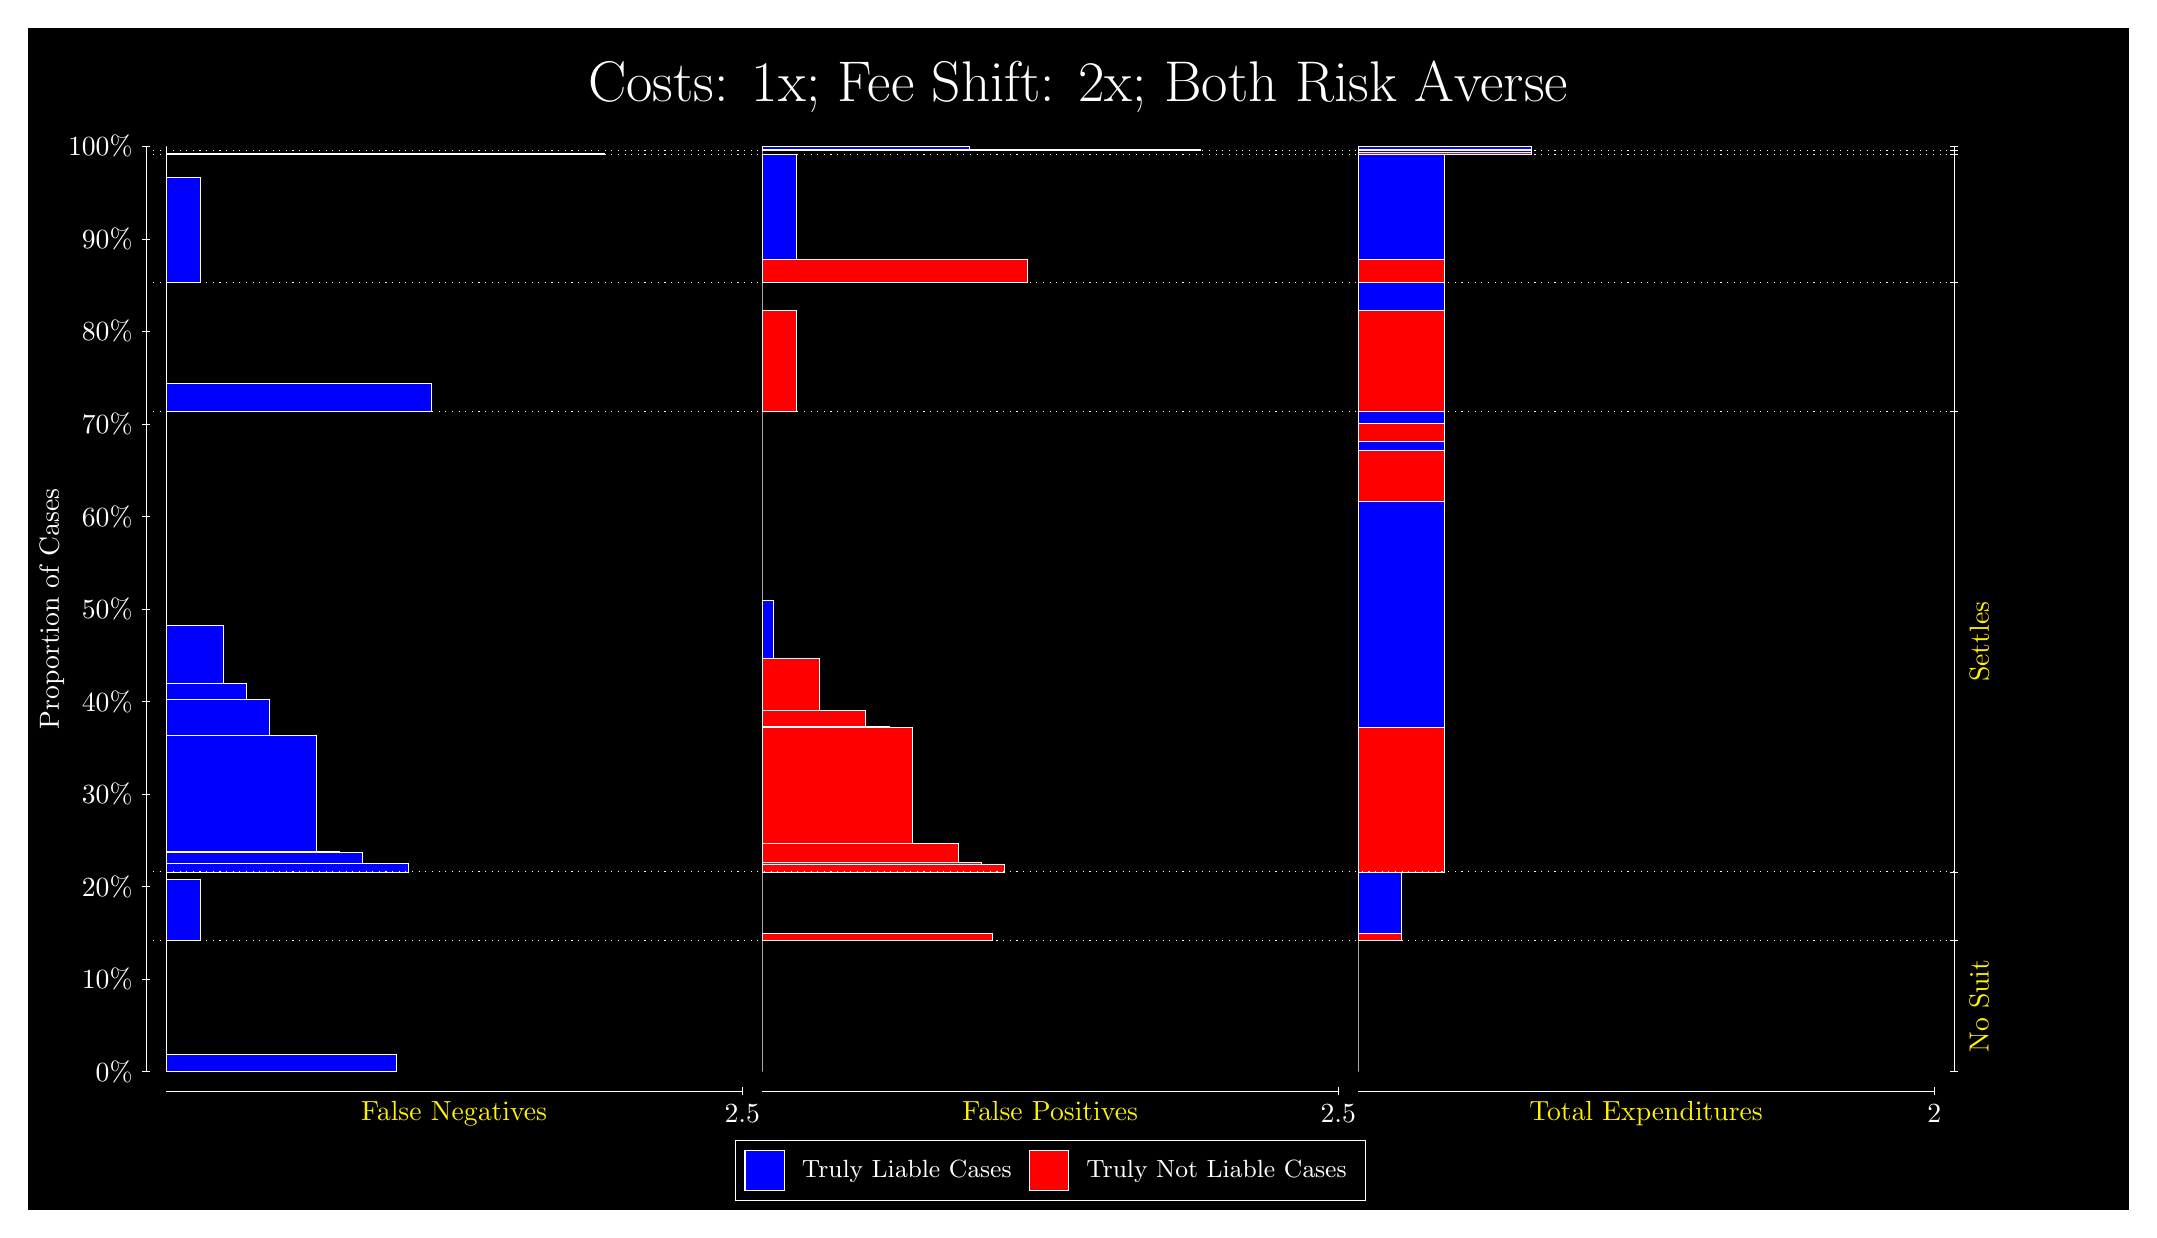
\begin{tikzpicture}
\draw[fill=black] (0,0) rectangle (26.667,15);
\draw[text=white] (0,13.5) rectangle (26.667,15) node[midway] {\huge Costs: 1x; Fee Shift: 2x; Both Risk Averse};
\draw[white, very thin] (1.5,1.75) -- (1.5,13.5);
\node[rotate=90, text=white, anchor=center] at (0.3, 7.625) {Proportion of Cases};
\draw[white, very thin] (1.45,1.75) -- (1.55,1.75);
\node[text=white, anchor=east] at (1.45, 1.75) {0\%};
\draw[white, very thin] (1.45,2.925) -- (1.55,2.925);
\node[text=white, anchor=east] at (1.45, 2.925) {10\%};
\draw[white, very thin] (1.45,4.1) -- (1.55,4.1);
\node[text=white, anchor=east] at (1.45, 4.1) {20\%};
\draw[white, very thin] (1.45,5.275) -- (1.55,5.275);
\node[text=white, anchor=east] at (1.45, 5.275) {30\%};
\draw[white, very thin] (1.45,6.45) -- (1.55,6.45);
\node[text=white, anchor=east] at (1.45, 6.45) {40\%};
\draw[white, very thin] (1.45,7.625) -- (1.55,7.625);
\node[text=white, anchor=east] at (1.45, 7.625) {50\%};
\draw[white, very thin] (1.45,8.8) -- (1.55,8.8);
\node[text=white, anchor=east] at (1.45, 8.8) {60\%};
\draw[white, very thin] (1.45,9.975) -- (1.55,9.975);
\node[text=white, anchor=east] at (1.45, 9.975) {70\%};
\draw[white, very thin] (1.45,11.15) -- (1.55,11.15);
\node[text=white, anchor=east] at (1.45, 11.15) {80\%};
\draw[white, very thin] (1.45,12.325) -- (1.55,12.325);
\node[text=white, anchor=east] at (1.45, 12.325) {90\%};
\draw[white, very thin] (1.45,13.5) -- (1.55,13.5);
\node[text=white, anchor=east] at (1.45, 13.5) {100\%};

\draw[white, very thin] (24.457,1.75) -- (24.457,13.5);
\draw[white, very thin] (24.407,1.75) -- (24.507,1.75);
\node[anchor=west] at (24.407, 1.75) {};
\draw[white, very thin] (24.407,3.4108) -- (24.507,3.4108);
\node[anchor=west] at (24.407, 3.4108) {};
\draw[white, very thin] (24.407,4.2853) -- (24.507,4.2853);
\node[anchor=west] at (24.407, 4.2853) {};
\draw[white, very thin] (24.407,10.131) -- (24.507,10.131);
\node[anchor=west] at (24.407, 10.131) {};
\draw[white, very thin] (24.407,11.775) -- (24.507,11.775);
\node[anchor=west] at (24.407, 11.775) {};
\draw[white, very thin] (24.407,13.398) -- (24.507,13.398);
\node[anchor=west] at (24.407, 13.398) {};
\draw[white, very thin] (24.407,13.446) -- (24.507,13.446);
\node[anchor=west] at (24.407, 13.446) {};
\draw[white, very thin] (24.407,13.5) -- (24.507,13.5);
\node[anchor=west] at (24.407, 13.5) {};

\draw[white, very thin, fill=blue] (1.75,1.75) rectangle (4.6775,1.9686);
\draw[white, very thin, fill=red] (1.75,1.9686) rectangle (1.75,3.4108);
\draw[white, very thin, fill=blue] (1.75,3.4108) rectangle (2.1891,4.1933);
\draw[white, very thin, fill=red] (1.75,4.1933) rectangle (1.75,4.2853);
\draw[white, very thin, fill=blue] (1.75,4.2853) rectangle (4.8239,4.3937);
\draw[white, very thin, fill=blue] (1.75,4.3937) rectangle (4.2384,4.536);
\draw[white, very thin, fill=blue] (1.75,4.536) rectangle (3.9457,4.5467);
\draw[white, very thin, fill=blue] (1.75,4.5467) rectangle (3.6529,6.0174);
\draw[white, very thin, fill=blue] (1.75,6.0174) rectangle (3.0674,6.4837);
\draw[white, very thin, fill=blue] (1.75,6.4837) rectangle (2.7746,6.6795);
\draw[white, very thin, fill=blue] (1.75,6.6795) rectangle (2.4819,7.418);
\draw[white, very thin, fill=red] (1.75,7.418) rectangle (1.75,10.131);
\draw[white, very thin, fill=blue] (1.75,10.131) rectangle (5.1167,10.485);
\draw[white, very thin, fill=red] (1.75,10.485) rectangle (1.75,11.775);
\draw[white, very thin, fill=blue] (1.75,11.775) rectangle (2.1891,13.107);
\draw[white, very thin, fill=red] (1.75,13.107) rectangle (1.75,13.398);
\draw[white, very thin, fill=blue] (1.75,13.398) rectangle (7.3123,13.415);
\draw[white, very thin, fill=red] (1.75,13.415) rectangle (1.75,13.446);
\draw[white, very thin, fill=red] (1.75,13.446) rectangle (1.75,13.463);
\draw[white, very thin, fill=blue] (1.75,13.463) rectangle (1.75,13.5);
\draw[white, very thin, fill=red] (9.3189,1.75) rectangle (9.3189,3.1923);
\draw[white, very thin, fill=blue] (9.3189,3.1923) rectangle (9.3189,3.4108);
\draw[white, very thin, fill=red] (9.3189,3.4108) rectangle (12.246,3.5028);
\draw[white, very thin, fill=blue] (9.3189,3.5028) rectangle (9.3189,4.2853);
\draw[white, very thin, fill=red] (9.3189,4.2853) rectangle (12.393,4.3857);
\draw[white, very thin, fill=red] (9.3189,4.3857) rectangle (12.1,4.4124);
\draw[white, very thin, fill=red] (9.3189,4.4124) rectangle (11.807,4.6476);
\draw[white, very thin, fill=red] (9.3189,4.6476) rectangle (11.222,6.1164);
\draw[white, very thin, fill=red] (9.3189,6.1164) rectangle (10.929,6.1309);
\draw[white, very thin, fill=red] (9.3189,6.1309) rectangle (10.636,6.3424);
\draw[white, very thin, fill=red] (9.3189,6.3424) rectangle (10.051,6.9981);
\draw[white, very thin, fill=blue] (9.3189,6.9981) rectangle (9.4652,7.7366);
\draw[white, very thin, fill=blue] (9.3189,7.7366) rectangle (9.3189,10.131);
\draw[white, very thin, fill=red] (9.3189,10.131) rectangle (9.758,11.42);
\draw[white, very thin, fill=blue] (9.3189,11.42) rectangle (9.3189,11.775);
\draw[white, very thin, fill=red] (9.3189,11.775) rectangle (12.686,12.065);
\draw[white, very thin, fill=blue] (9.3189,12.065) rectangle (9.758,13.398);
\draw[white, very thin, fill=red] (9.3189,13.398) rectangle (9.3189,13.429);
\draw[white, very thin, fill=blue] (9.3189,13.429) rectangle (9.3189,13.446);
\draw[white, very thin, fill=red] (9.3189,13.446) rectangle (14.881,13.463);
\draw[white, very thin, fill=blue] (9.3189,13.463) rectangle (11.954,13.5);
\draw[white, very thin, fill=red] (16.888,1.75) rectangle (16.888,3.1923);
\draw[white, very thin, fill=blue] (16.888,3.1923) rectangle (16.888,3.4108);
\draw[white, very thin, fill=red] (16.888,3.4108) rectangle (17.437,3.5028);
\draw[white, very thin, fill=blue] (16.888,3.5028) rectangle (17.437,4.2853);
\draw[white, very thin, fill=red] (16.888,4.2853) rectangle (17.986,6.1164);
\draw[white, very thin, fill=blue] (16.888,6.1164) rectangle (17.986,8.9876);
\draw[white, very thin, fill=red] (16.888,8.9876) rectangle (17.986,9.6433);
\draw[white, very thin, fill=blue] (16.888,9.6433) rectangle (17.986,9.7517);
\draw[white, very thin, fill=red] (16.888,9.7517) rectangle (17.986,9.9777);
\draw[white, very thin, fill=blue] (16.888,9.9777) rectangle (17.986,10.131);
\draw[white, very thin, fill=red] (16.888,10.131) rectangle (17.986,11.42);
\draw[white, very thin, fill=blue] (16.888,11.42) rectangle (17.986,11.775);
\draw[white, very thin, fill=red] (16.888,11.775) rectangle (17.986,12.065);
\draw[white, very thin, fill=blue] (16.888,12.065) rectangle (17.986,13.398);
\draw[white, very thin, fill=red] (16.888,13.398) rectangle (19.083,13.429);
\draw[white, very thin, fill=blue] (16.888,13.429) rectangle (19.083,13.446);
\draw[white, very thin, fill=red] (16.888,13.446) rectangle (19.083,13.463);
\draw[white, very thin, fill=blue] (16.888,13.463) rectangle (19.083,13.5);
\draw[white, dotted] (1.5,3.4108) -- (24.457,3.4108);
\draw[white, dotted] (1.5,4.2853) -- (24.457,4.2853);
\draw[white, dotted] (1.5,10.131) -- (24.457,10.131);
\draw[white, dotted] (1.5,11.775) -- (24.457,11.775);
\draw[white, dotted] (1.5,13.398) -- (24.457,13.398);
\draw[white, dotted] (1.5,13.446) -- (24.457,13.446);
\draw[white, very thin] (1.75,1.5) -- (9.0689,1.5);
\node[text=yellow, anchor=north] at (5.4094, 1.5) {False Negatives};
\draw[white, very thin] (9.0689,1.45) -- (9.0689,1.55);
\node[text=white, anchor=north] at (9.0689, 1.45) {2.5};

\draw[white, very thin] (9.3189,1.5) -- (16.638,1.5);
\node[text=yellow, anchor=north] at (12.978, 1.5) {False Positives};
\draw[white, very thin] (16.638,1.45) -- (16.638,1.55);
\node[text=white, anchor=north] at (16.638, 1.45) {2.5};

\draw[white, very thin] (16.888,1.5) -- (24.207,1.5);
\node[text=yellow, anchor=north] at (20.547, 1.5) {Total Expenditures};
\draw[white, very thin] (24.207,1.45) -- (24.207,1.55);
\node[text=white, anchor=north] at (24.207, 1.45) {2};

\node[text=yellow, centered, rotate=90] at (24.777, 2.5804) {No Suit};

\node[text=yellow, centered, rotate=90] at (24.777, 7.208) {Settles};





\draw (12.978300999999998,1.5) node[draw=none] (baseCoordinate) {};
\begin{scope}[align=center]
        \matrix[scale=0.5, draw=white, below=0.5cm of baseCoordinate, nodes={draw}, column sep=0.1cm]{
            \node[rectangle, draw, minimum width=0.5cm, minimum height=0.5cm, fill=blue] {}; &
            \node[draw=none, font=\small, text=white] (B) {Truly Liable Cases}; &
            \node[rectangle, draw, minimum width=0.5cm, minimum height=0.5cm, fill=red] {}; &
            \node[draw=none, font=\small, text=white] (B) {Truly Not Liable Cases}; \\
            };
\end{scope}

\end{tikzpicture}
\end{document}